\documentclass{article}

% if you need to pass options to natbib, use, e.g.:
%     \PassOptionsToPackage{numbers, compress}{natbib}
% before loading neurips_2018

% ready for submission
% \usepackage{neurips_2018}

% to compile a preprint version, e.g., for submission to arXiv, add add the
% [preprint] option:
%     \usepackage[preprint]{neurips_2018}

% to compile a camera-ready version, add the [final] option, e.g.:
     \usepackage[final]{../templates/neurips_2018}

% to avoid loading the natbib package, add option nonatbib:
%     \usepackage[nonatbib]{neurips_2018}

\usepackage[utf8]{inputenc} % allow utf-8 input
\usepackage[T1]{fontenc}    % use 8-bit T1 fonts
\usepackage{hyperref}       % hyperlinks
\usepackage{url}            % simple URL typesetting
\usepackage{booktabs}       % professional-quality tables
\usepackage{amsfonts}       % blackboard math symbols
\usepackage{nicefrac}       % compact symbols for 1/2, etc.
\usepackage{microtype}      % microtypography

\usepackage{wrapfig}
\usepackage{graphicx, subcaption}		% images

\usepackage{xcolor}

\captionsetup[sub]{font=tiny,labelfont={bf,sf}}
\DeclareCaptionFont{tiny}{\tiny} 
\captionsetup{font+=scriptsize} 
\captionsetup[sub]{font+=tiny}
\captionsetup{labelfont=bf}



\renewcommand{\arraystretch}{1.2}



\title{Evaluating QANet on SQuAD 2.0}

% The \author macro works with any number of authors. There are two commands
% used to separate the names and addresses of multiple authors: \And and \AND.
%
% Using \And between authors leaves it to LaTeX to determine where to break the
% lines. Using \AND forces a line break at that point. So, if LaTeX puts 3 of 4
% authors names on the first line, and the last on the second line, try using
% \AND instead of \And before the third author name.

\author{%
  Parthasarathy Suryanarayanan\\
   \texttt{psuryan@stanford.edu} \\
  \And
  Yash Mangilal Jain\\
  \texttt{yashjain@stanford.edu} \\
  % examples of more authors
  % \And
  % Coauthor \\
  % Affiliation \\
  % Address \\
  % \texttt{email} \\
  % \AND
  % Coauthor \\
  % Affiliation \\
  % Address \\
  % \texttt{email} \\
  % \And
  % Coauthor \\
  % Affiliation \\
  % Address \\
  % \texttt{email} \\
  % \And
  % Coauthor \\
  % Affiliation \\
  % Address \\
  % \texttt{email} \\
}

\begin{document}
% \nipsfinalcopy is no longer used

\maketitle

\begin{abstract}
\small
The QANet architecture \cite{yu2018qanet} was evaluated against the SQuAD [1.1] dataset \citep{rajpurkar2016squad} with impressive results (EM: 82.47 and F1: 89.30). The SQuAD [2.0] dataset \cite{rajpurkar2018know}, the latest revision of SQuAD, tests the ability of a system to not only answer the question whenever possible but also determine when no answer is supported by the paragraph and abstain from answering. Thus, it poses a much more challenging machine comprehension task. The main objective of this work is to evaluate the QANet system on  the SQuAD [2.0] dataset, by implementing the architecture from the ground up and to understand the challenges posed by the non-answerability. 
\end{abstract}

\section{Introduction}
\small
We can define machine comprehension in terms of Question Answering in its most general form \cite{burges2013towards}.  Recently a variety of neural architectures have achieved near-human performance in open domain question answering tasks. These recent advances are broadly of two types – (1) Pre-trained Contextual Embeddings (PCE) based methods such as ELMo\cite{peters2018deep}, Bert\cite{devlin2018bert} etc. and (2) Non-PCE methods. The former offers more of an “off-the-shelf” module that could be employed for specific tasks such as question answering, the latter, even though not being the state of the art (SoTA) any longer (as of Feb 2019), offer more scope for creativity and opportunities for deep learning practitioners to explore different techniques and develop intuitions behind them. One of the successful non-PCE approaches to machine comprehension is the QANet architecture.  

The main goal of the QANet architecture is efficiency / speed which also results in performance gain as a nice by-product. The authors of the system demonstrate the efficiency and performance improvements on SQuAD [1.1] dataset. However, suitability of the architecture for the non-answerability setting has not been systematically evaluated to our knowledge. Our major focus is understanding the limitations of QANet against SQuAD [2.0] dataset and investigating methods to augment the architecture, to predict if the question can be answered or not based on the information from the comprehension.

The organization of the paper is as follows. In Section 2 we briefly show the landscape of related work. Section 3 gives a comprehensive overview of the QANet architecture and our approach for implementation. Section 4 describes the different experiments we conducted. Section 5 discusses our observations. In Section 6, we summarize our main conclusions from this work and describe our vision for the future.

\section{Related Work}
\small
Prior to QANet, major question answering systems primarily contained either of two key ingredients (1) recurrent units such as LSTM for capturing sequential input and (2) exploiting attention mechanism for capturing long-term interactions. For example, popular non-PCE models such as, Multi-Paragraph Reading Comprehension \cite{clark2017simple}, Gated Self-Matching Networks (R-Net) \cite{wang2017gated} and Match-LSTM \cite{wang2016machine} use these ideas. The BiDAF \cite{seo2016bidirectional} model which we use as the baseline, employs both the techniques, is a hierarchical multi-stage end-to-end network which takes inputs of different granularity (character, word and  phrase) to obtain a query-aware context representation using memory-less context-to-query (C2Q) and query-to-context (Q2C) attention. This representation can then be used for different final tasks, such as question answering. 

However, due to the sequential nature, (1) can’t be parallelized to exploit the hardware and hence is slow. To achieve the speedup, the QANet borrows a neat idea from NMT, proposed in the Transformer\cite{vaswani2017attention} architecture: encode the question and context separately using a non-recurrent, therefore faster, encoder. This encoder uses convolution (which models the local features) and self-attention (which models global interaction) as building blocks. The parallel nature of CNN architectures leads to a significant speed boost, especially given the fact that context passages in SQuAD are really long.

\section{Approach}
\small
The first of our two step approach is essentially implementing the architecture carefully as specified in the paper. The second step is to perform an error analysis on the development set, understand the strengths and weaknesses of the model come up with a few ideas that might help the performance. We describe the QANet architecture in the following section at a high level. Please refer to the original paper \cite{yu2018qanet} for details. 

\subsection{Representation}
\small
Before we dive deep into the architecture, it is useful to define the terminology and representation. Recall that the QA problem can succinctly be formulated as following: Given 
	a context / passage of n words, $C = \{c_1,c_2...,c_n\}$
	and a question / query sentence of m words, $Q = \{q_1,q_2...,q_m\}$,
we want to output a span $S=\{c_i,c_{{i+1}},...c_{{i+j}}\}$ from the original paragraph C if the question is answerable. QANet uses fixed size contexts and questions. In the default implementation, only the first 400 tokens in the given paragraphs are used as context and 50 tokens in the given question are used as  query. For each word, first 16 characters are only used to compute the character embeddings. If the context/query is shorter than the length threshold, zero-padding is applied. QANet uses pre-trained GloVe \cite{pennington2014glove} vectors as word and character embeddings for representing both query and context. 

\subsection{Model}
\small

\begin{figure}[h]
  \vspace{-10pt}
  \centering
  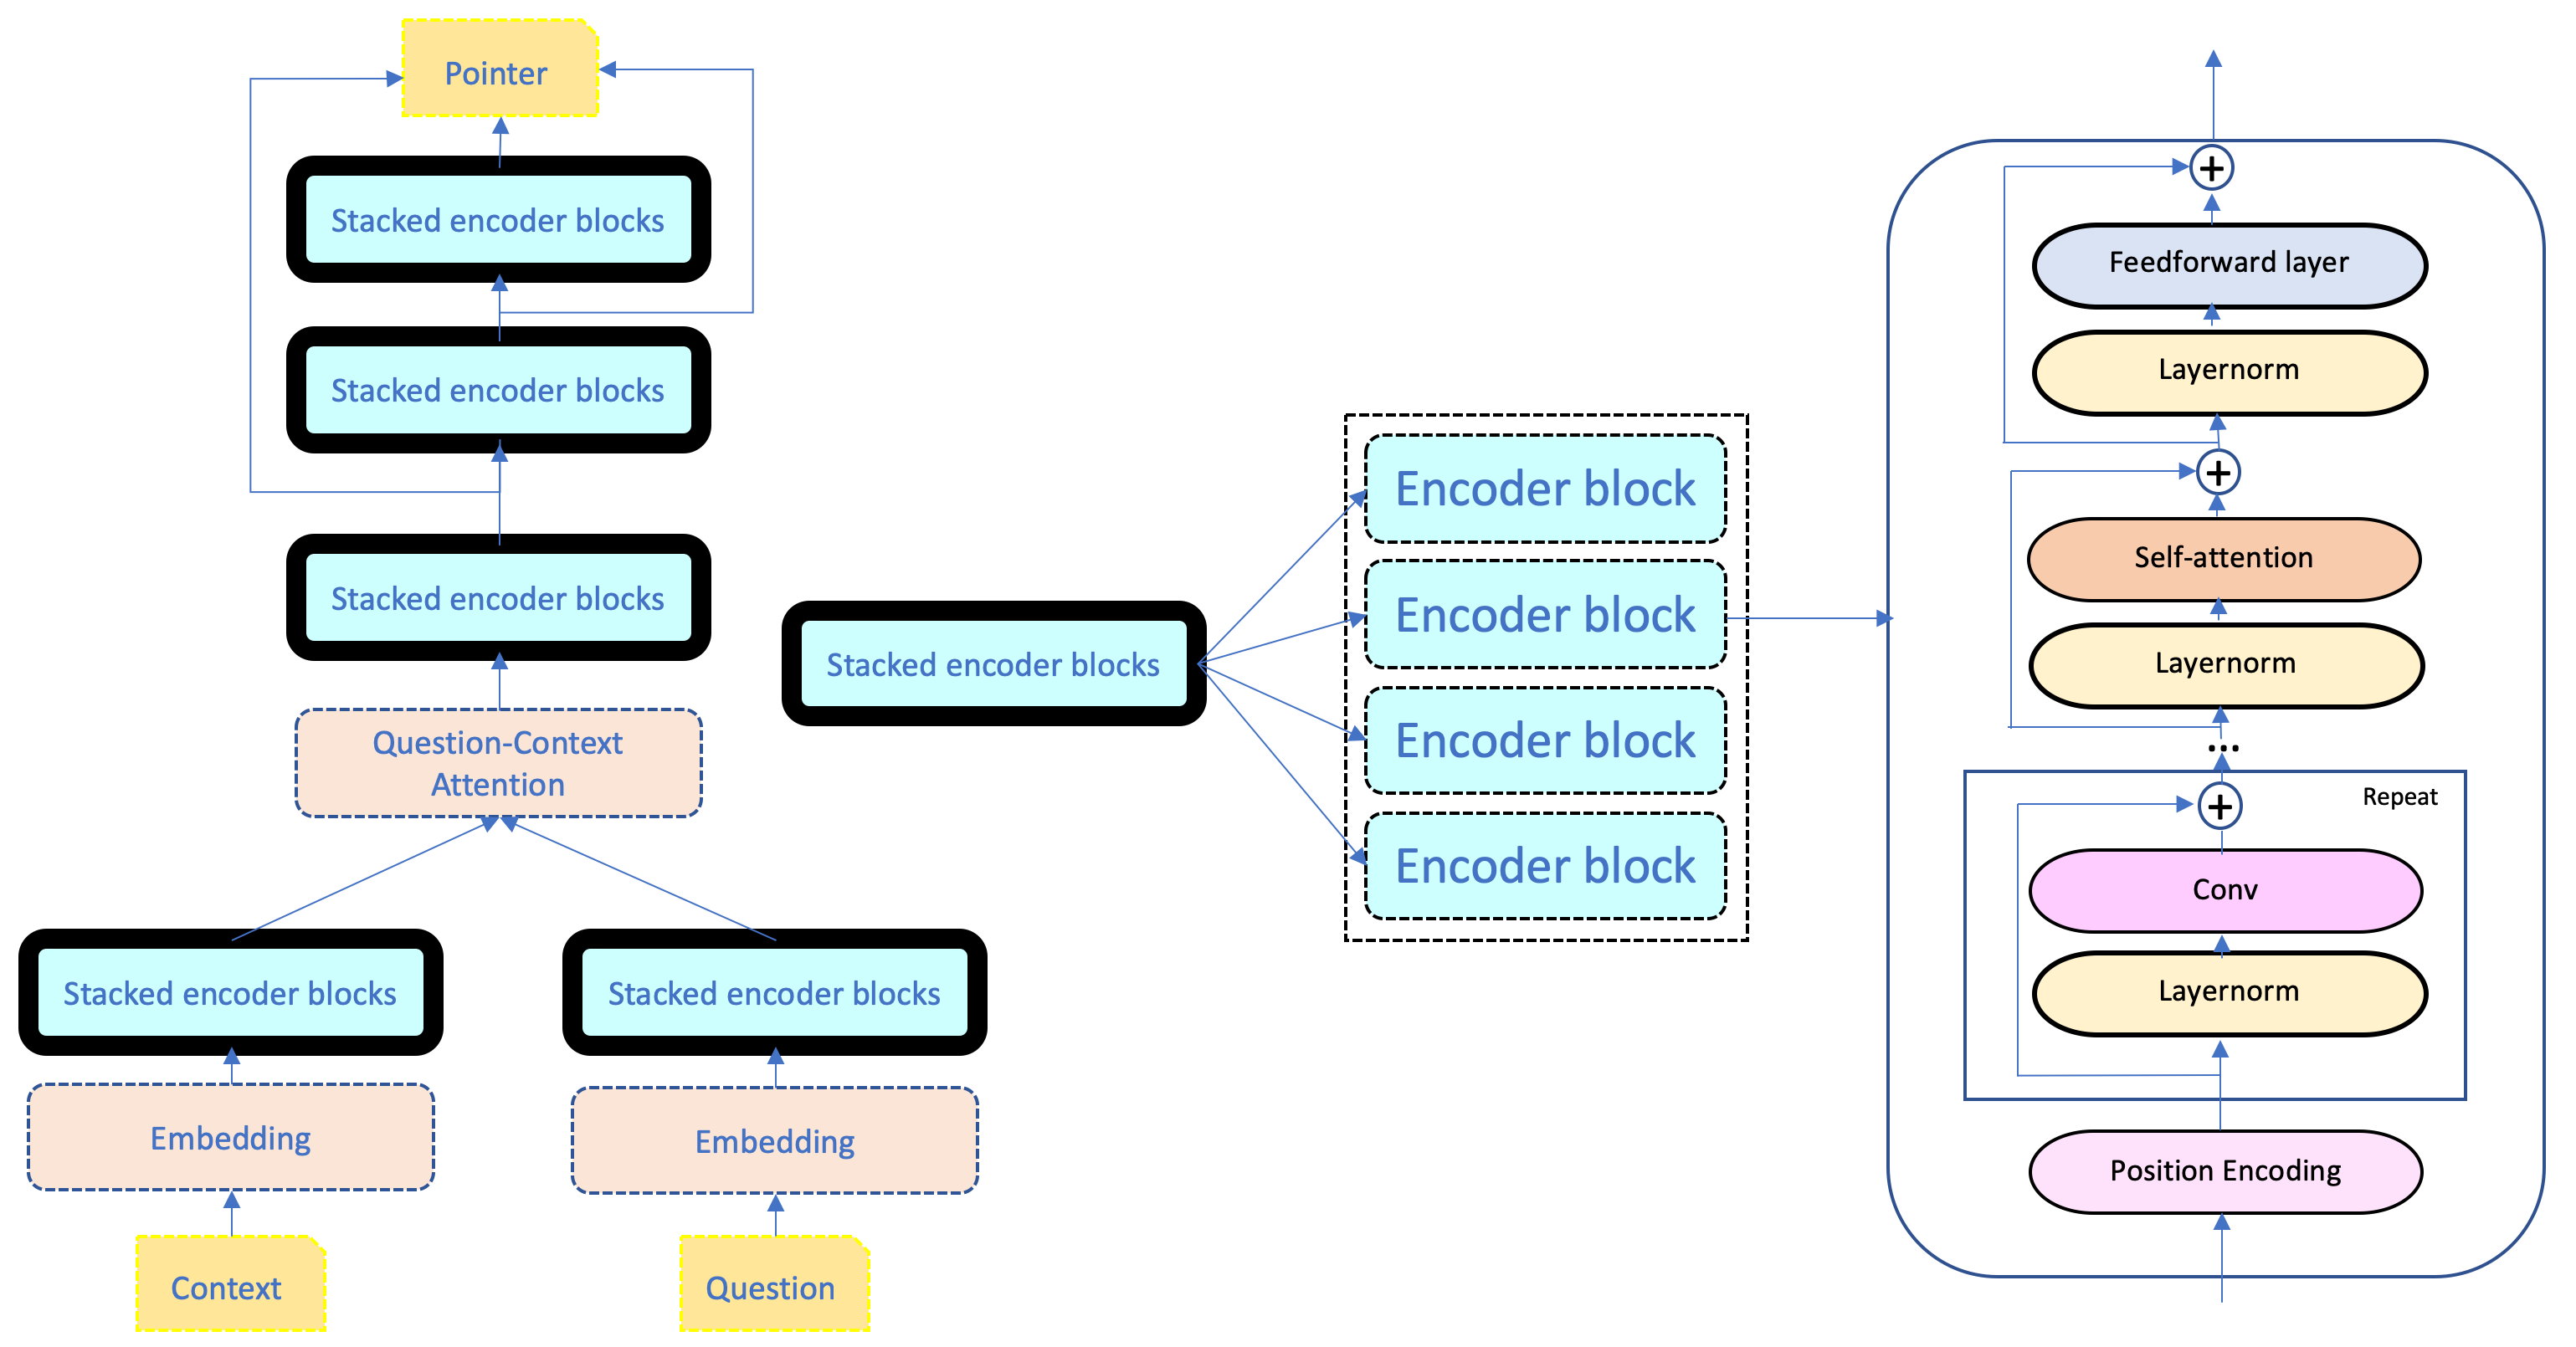
\includegraphics[width=0.5\linewidth]{../images/qanet_architecture.png}
    \caption{Model}
      \label{model-figure}
\end{figure} 
QANet architecture, shown in Figure~\ref{model-figure}. But before we examine the layers, we need to look at a key component that is used in several places with the model, the encoder block. The encoder block draws upon many ideas from the Transformer \cite{vaswani2017attention}. It is stacked several times and the stack is used in three different places: to encode the question, to encode the context and finally on encode the model 3 times. 
The encoder block consists of four key layers.
\begin{enumerate}
  \item {\textit{Positional embedding layer:} The position of a word within a sentence carries useful information for the model. In an RNN, this information is trivially encoded as the inputs are presented to the model one step at time. But for non-RNN model, a “positional encoding” is needed to be given explicitly. This layer adds the positional encoding to the input at the beginning of each encoder layer as defined in Transformer}
  \item {\textit{Convolution layer:} This is repeated multiple times and the number varies based on the location of usage of the encounter block. the implementation uses depth-wise separable convolutions \cite{chollet2017xception} which require an order of magnitude less computation to achieve nearly the same result as the normal convolution. This is a key ingredient of the speedup. (Details: kernel / filter size: 7, number of filters: 128)}
  \item {\textit{Self-attention layer:} the multi-head attention mechanism, again from Transformer is used with number of attention heads as 8. Attention key depth is 128 and depth per head is 16.}
  \item {\textit{Feed-Forward layer}}
\end{enumerate}

The model consists of 5 key modules: an embedding layer, an encoder layer, a context-query attention layer, a modeling layer and an output layer.  

\begin{enumerate}
  \item {\textbf{Embedding layer:} combines the word and character embeddings into a singular representation for each word. This is done by, }
	\begin{enumerate}  
		\item Looking up the 300 ($p1$) dimensional pre-trained GloVe embeddings $[x_w]$
		\item {Learning a 200 ($p2$) dimensional embedding for each character in the word using convolution $[x_c]$. The character embeddings are passed through a convolutional layer and a max-pooling layer, as described in \cite{kim2014convolutional}, to produce 200-dimensional character-level word embeddings. The intuition behind using a character-level embedding is to be able to handle out of vocabulary words (OOV), rare words, misspellings and morphology during test time.}
		\item Concatenating the two vectors into $[x_w; x_c]$ into a vector of size  $(p1+p2)$. Also, a two-layer highway network \cite{srivastava2015highway} is also used as optimization to avoid the vanishing gradient problem.
	\end{enumerate}
  
  \item {\textbf{Encoder layer:} After that, the context and the question are passed through encoder layer. This layer uses a single encoder block with 4 convolutions. The output of this layer is of 128 dimensions $(hidden\_size)$ as the input is immediately converted to this dimension by a one-dimensional convolution. \textbf{Note:} In our implementation, we convolved down from 500 dimension to $hidden\_size$ in the embedding layer itself.}
  \item {\textbf{Context-Query Attention layer:} The output from the encoders are fed to the Context-Query attention layer which combines context and query and produces a representation for each word in context. This is similar to the previous reading comprehension models, such as \cite{weissenborn2017making} and \cite{chen2017reading}. The purpose of this layer is to calculate two quantities.}
  	\begin{enumerate}  
	\item \textit{Context-to-query attention ($A$):} First calculate pair wise similarities between words in the encoded context ($C$) and encoded query ($Q$). The similarity measure is a trilinear function as described in \cite{weissenborn2017making} $f(q,c)= W0[q,c, q \odot c]$. This would yield a matrix $S$ of dimensions $n$ x $m$. $W0$ is a trainable variable. After normalizing each row using $softmax$, we get a different matrix $\overline S$. The context-to-query-attention is calculated as $A = \overline S \cdot Q^T$
	\item \textit{Query-to-context attention ($B$):} Column-normalizing $S$ yields $\overline {\overline S}$. The query-to-context attention is calculated as $B = S \cdot \overline {\overline S} ^T \cdot C^T$
	\end{enumerate}  
	\item \textbf{Model encoder layer:} The input to this layer at each position is $c,a,c \odot a,c \odot b$ where $a$ and $b$ are rows from attention matrices $A$ and $B$ calculated above. This layer consists of 3 stacked encoder blocks that share weights and the number of encoder blocks within each stack is 7. The number of convolutions within each block is 2.
	\item \textbf{Output layer:} The key layer for prediction is the output layer. Similar to method described in \cite{seo2016bidirectional}, the optimization function is formulated as follows. Let $$P^1 = \textit{softmax}(W_1[M_0 ; M_1]) \qquad P^2 = \textit{softmax}(W_2[M_0 ; M_2])$$ be the probabilities of each position in the context being start and end of the answer span, respectively. Where $W_1$ and $W_2$ are trainable weights and $M_0 , M_1 , M_2$ are outputs from the three model encoders. Now the objective function could be defined as the sum of negative log probabilities of predicted distributions indexed by true start and end indices, averaged over the training instances. $$Log(\theta) = - 1/N \sum_i^N [log(P^1_{{y^1_i}}) + (P^2_{{y^2_i}})]$$
Where $y_i^1$ and $y_i^2$ are start end positions of the $i^{{th}}$  training instance from ground truth. The model outputs probabilities for all pairs similar to other pointer networks for reading comprehension. Through an efficient method (such as using dynamic programming), the best pair of spans $(s,e)$ that maximize $p_s^1 p_e^1$ have to be chosen as the prediction. Ultimately these probabilities are turned into a span consisting of a start index and an end index, indicating the location of the answer in the context paragraphs. Since, the answer is essentially a contiguous phrase in the context, predicting start and end index is sufficient. 
\end{enumerate}	


\section{Experiments}

\subsection{Data}
We now describe the SQuAD [2.0] dataset\cite{rajpurkar2018know}, customized for default final project in more detail, starting with some general statistics. The training, development and test sets consist of 129941, 5951 and 5918 questions respectively. As noted earlier, the question and context are truncated to 50 and 400 tokens respectively. 
Since pure Transformer based architectures have been known not to do well on very long-range dependencies \cite{dai2019transformerxl}, we take note of the distribution of the context length for the development set in Figure~\ref{dataset-distributions-figure}


\begin{figure}[h]
  \vspace{-10pt}
  \centering
  \subcaptionbox{Context lengths}{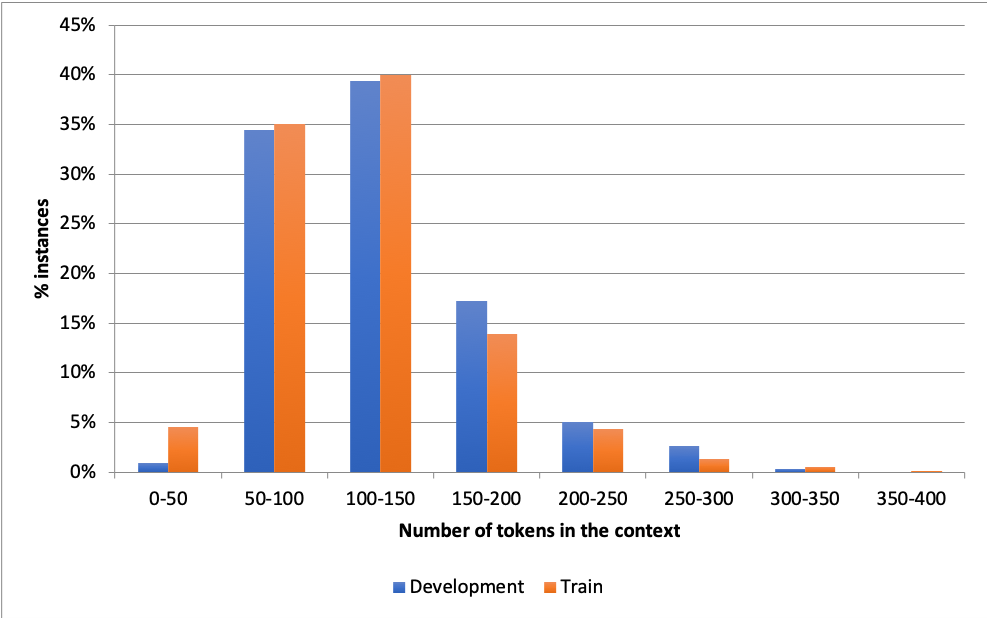
\includegraphics[height=7\baselineskip]{../images/fr_context_length.png}} \quad
  \subcaptionbox{Question categories}{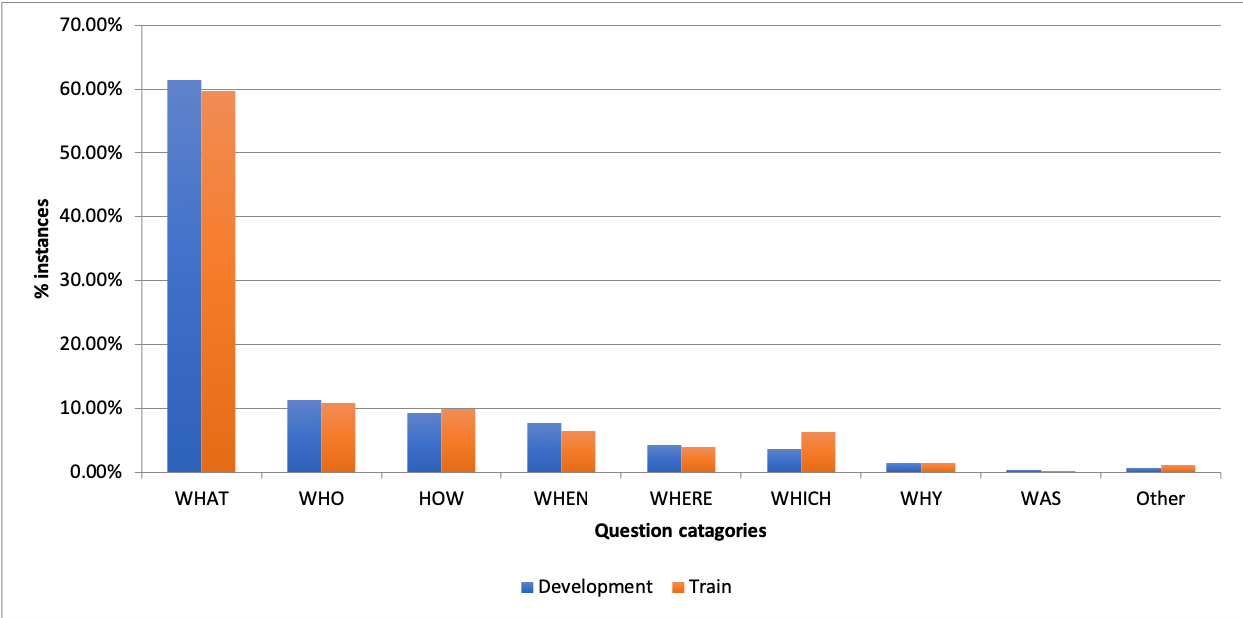
\includegraphics[height=7\baselineskip]{../images/fr_question_catagories.png}} \quad
  \caption{Dataset distributions} 
  \label{dataset-distributions-figure}
\end{figure}

The dataset contains approximately 50\% unanswerable questions due to a range of linguistic phenomena such as negation, antonyms, entity swapping etc. However, while the dataset provides high quality questions and answers, many of them tend to be of $wh-$ type. Figure~\ref{dataset-distributions-figure} shows the distribution of these question types. Also, there is some repetition of answers—of the 5951 questions in the development set 2848 questions are answerable (47.8\%) with 2596 distinct answers; there are 194 repeated answers (7.4\%).

\subsection{Evaluation}
We use the standard evaluation metrics for SQuAD - EM (Exact Match) and F1 measure. The baseline for our implementation is the Bi-DAF model supplied as part of the default final project. 

\subsection{Experiment detail}
\begin{figure}[h]
  \centering
  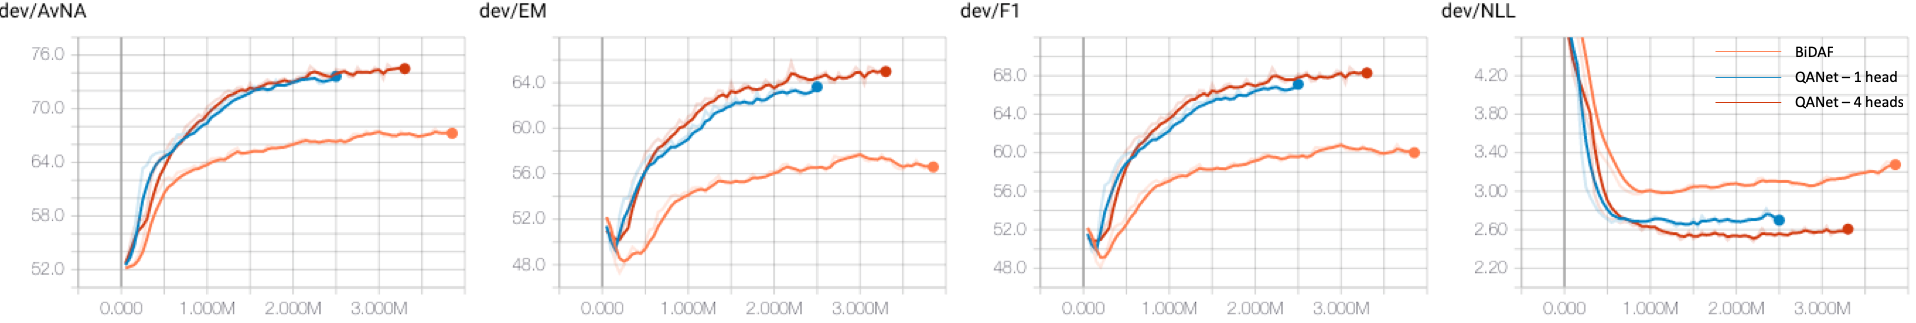
\includegraphics[width=\linewidth]{../images/fr_experiment.png}
  \caption{Experiments}
  \label{experiments-figure}
\end{figure} 
In this section, we describe the experiments conducted by us to evaluate the performance of the QANet model on the SQuAD [2.0] dataset. The Figure~\ref{experiments-figure} shows our main experimental runs. All the experiments were run with the hyper parameters specified in the paper except for the following changes. The $hidden\_size$ of the model was set to 96 instead of 128 due to hardware limitations. Our hyper-parameter search was limited to changes in number of heads for the multi-headed attention. We ran two experiments with 1 and 4 attention heads respectively. The hardware used for the experiment is NV6 class of GPU machines provided by Microsoft Azure with 8GB of video memory. It was observed that close 7.9GB was used. The baseline BiDAF model was run for 30 epochs. The two QANet experiments were manually stopped before 30 epochs upon observing the stabilization of dev NLL (negative log-likelihood loss). While the BiDAF was run with batch size of 64, the QANet was run with batch size of 32 due to memory constraints. The typical wall-clock time per epoch for the three models were 16, 53 and 80 minutes respectively. We found that variable context length batches (where sentences are padded to $max_len$) ran about 30\% (2) faster than padding all sentences across batches to 400 tokens.

Also, as specified in the paper, we use three different regularization techniques. 

\begin{enumerate}
  \item L2 weight decay on all trainable kernels with $\lambda = 3e^{-7}$.
  \item Dropout with $drop\_prob = 0.1$ after every other layer. Additionally dropout is applied word embedding and character embedding with $drop\_prob$ of 0.1 and 0.05 respectively.
  \item Stochastic depth dropout (layer dropout) on every sublayer in an Encoder Block. For an Encoder Block with $L$ total sublayers, during training, the $l-th$ sublayer has probability $p_l = 1 - (l/L) * drop\_prob$ of survival (i.e., earlier sublayers are more likely to survive). For the question and context encoders, $L = 6$. For each of the stacked encoder blocks within the model encoder, $L = 28$.
\end{enumerate}	

It is to be noted that as a departure from the QANet paper, we chose not to implement any data-augmentation due to time-constraints.

\subsection{Results}
Our model achieves competitive scores of $60.57/64.44$ of $EM$ and $F1$ respectively on test set, in the non-PCE SQuAD [2.0] leaderboard. Also, the model performs considerably well on the development set with the scores of $65.68/68.67 (EM / F1)$ in the leaderboard. The differences in development and test scores could be attributed to slight differences in data distribution as our implementation had the same hyper parameters as the paper. We failed to observe any dramatic speedup over BiDAF baseline. We suspect that this is due to a combination of memory-intensive nature of the architecture on our limited hardware and some suboptimal implementation.  

\section{Analysis}

\begin{wrapfigure}{r}{0.5\linewidth}
  \vspace{-10pt}
\centering
   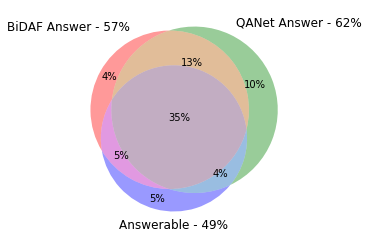
\includegraphics[width=\linewidth]{../images/Answerable.png}
\caption{Answerability prediction}
\label{answerable-figure}
\end{wrapfigure}

\textbf{Quantitative:} The main feature SQuAD [2.0] dataset is unanswerable questions. SQuAD [2.0] questions cannot be answered by learning simple heuristics such as word overlap or type matching \cite{rajpurkar2016squad}. To deal with unanswerable cases, systems must learn to identify a wide range of linguistic phenomena such as negation, antonymy and entity changes between the passage and the question. Therefore we expect the performance of the base QANet over SQuAD [2.0] to be worse than SQuAD [1.1]. Comparing the QANet results against the BiDAF (refer Figure~\ref{answerable-figure}), we find that QANet attempts to answer 62\% questions from the development set and predicts the answerability wrong 28\% of the time (6\% worse than BiDAF). Of these incorrect answerability predictions, the model is biased towards answering a question (23\%) rather than refraining (5\%). Based on this headroom, we note that any improvement answerability prediction will improve overall performance considerably.
The breakdown of correct answers (F1 > 0.5) by question categories is shown in Figure~\ref{f1_gt_0.5_question_catagories-figure}. Unsurprisingly the largest headroom lies in the \textit{What}-type questions.

\begin{wrapfigure}{r}{0.5\linewidth}
  \vspace{-15pt}
\centering
   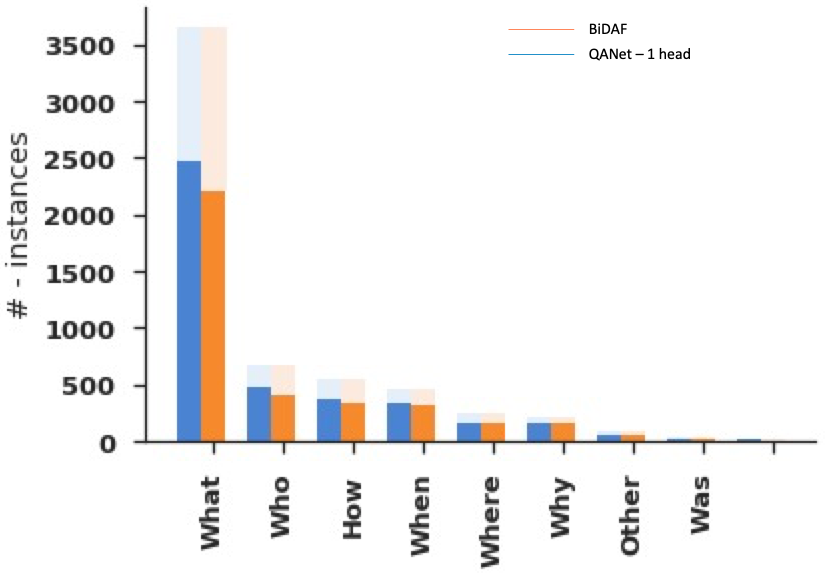
\includegraphics[width=\linewidth]{../images/f1gt5question_catagories.png}
\caption{Answer correctness (F1 > 0.5) by question category}
\label{f1_gt_0.5_question_catagories-figure}
\end{wrapfigure}




\textbf{Qualitative:} We randomly sampled 50 question of both answerable and unanswerable types separately and performed error analysis. Unfortunately due to time constraints, the error analysis was done on our initial set of results and not our best model (which was run with 4 attention heads). But we spot checked results from the best model and noted any changes. We identified a set of error categories. Also, we tried to identify the underlying root cause / different comprehension skills (co-reference etc.) needed by the the system as described in \cite{sugawara2017evaluation}. Breakdown of errors by category and skills are shown in  Figure~\ref{error-types-figure}. Examples for each error type and comprehension skill is shown in the Table~\ref{error-types-table}. 

We find that for the error cases where there is partial match on span, training a larger model (increased number of attention heads, bigger $hidden\_size$ etc.) reduces the error. In fact this is the largest error category (48\%). Only when there is no answer predicted by the model or when the answer is completely incorrect, we categorize the error by the deficiency in comprehension skill. In addition to the skills defined in \cite{sugawara2017evaluation} we added two categories: \textit{Long context} and \textit{Paraphrasing} as these did not fit into skillset. 

\begin{figure}[h]
  \centering
  \subcaptionbox{Error categories}{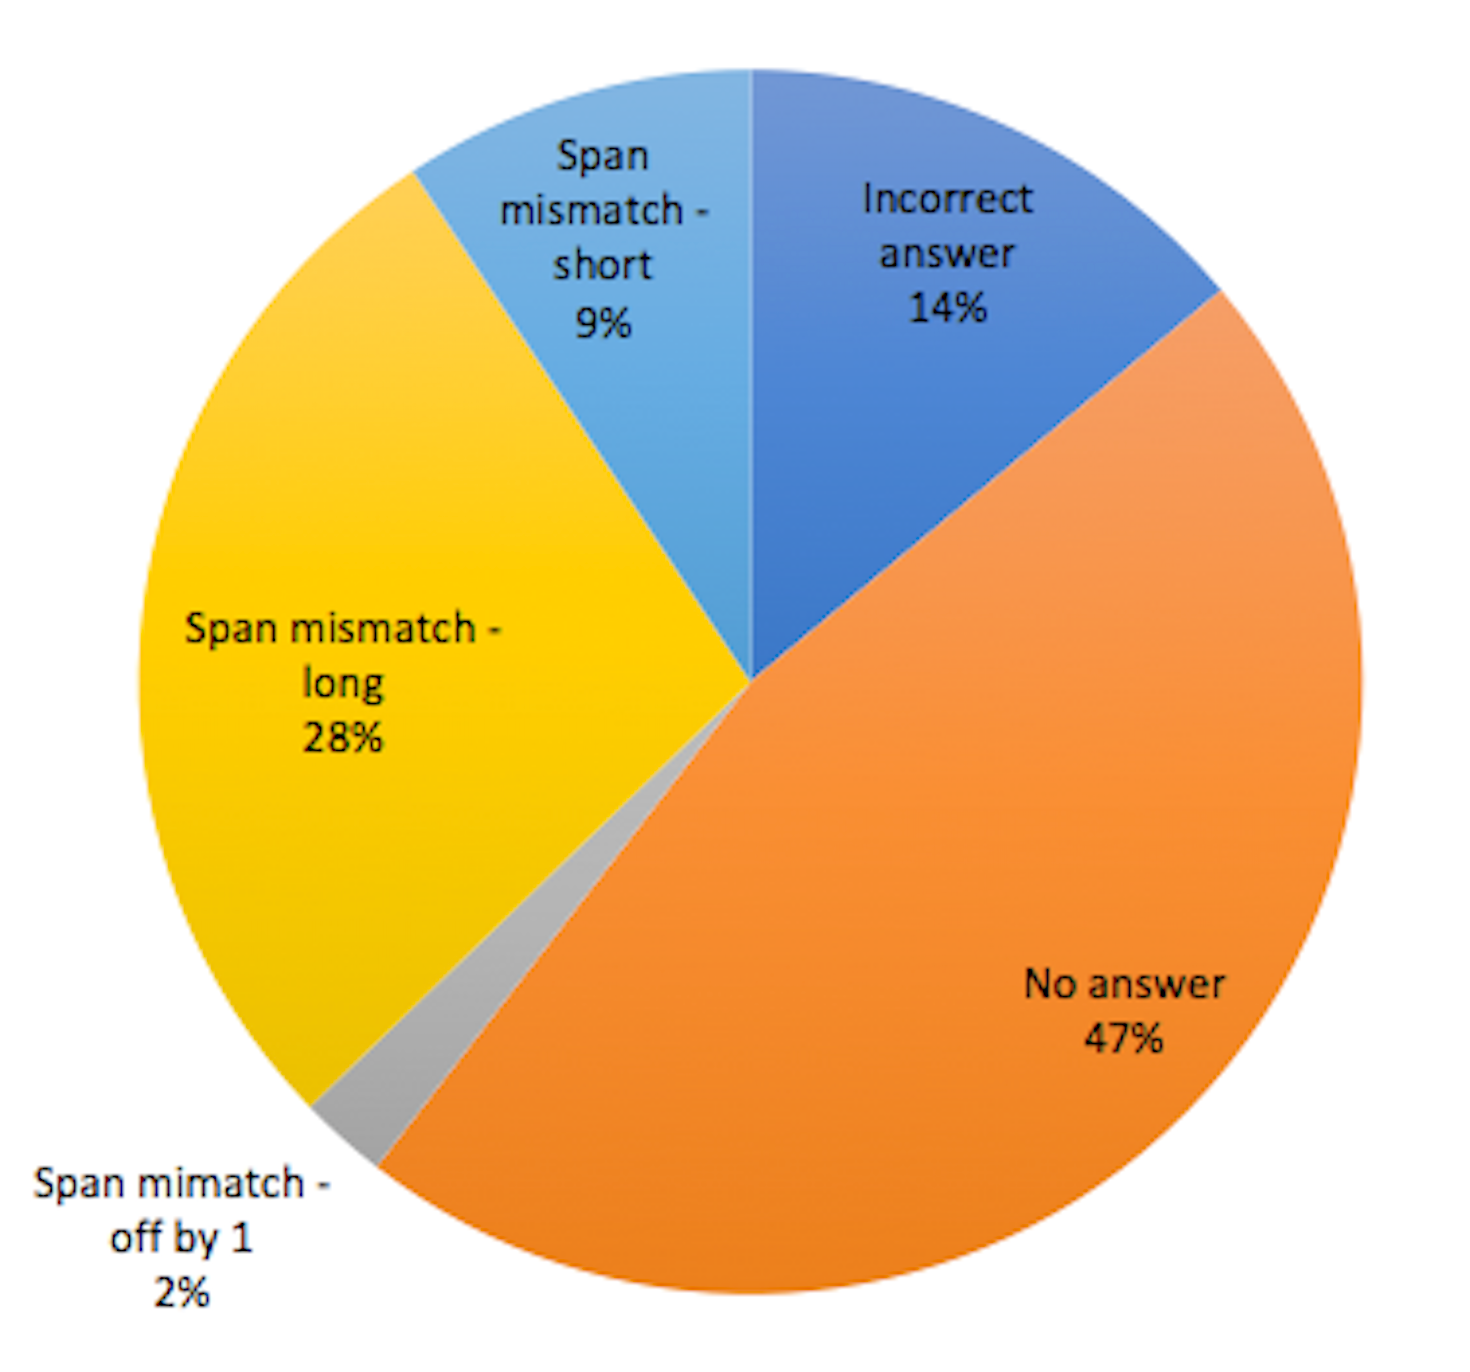
\includegraphics[height=10\baselineskip]{../images/error_types.png}} \quad
  \subcaptionbox{Skill deficiencies}{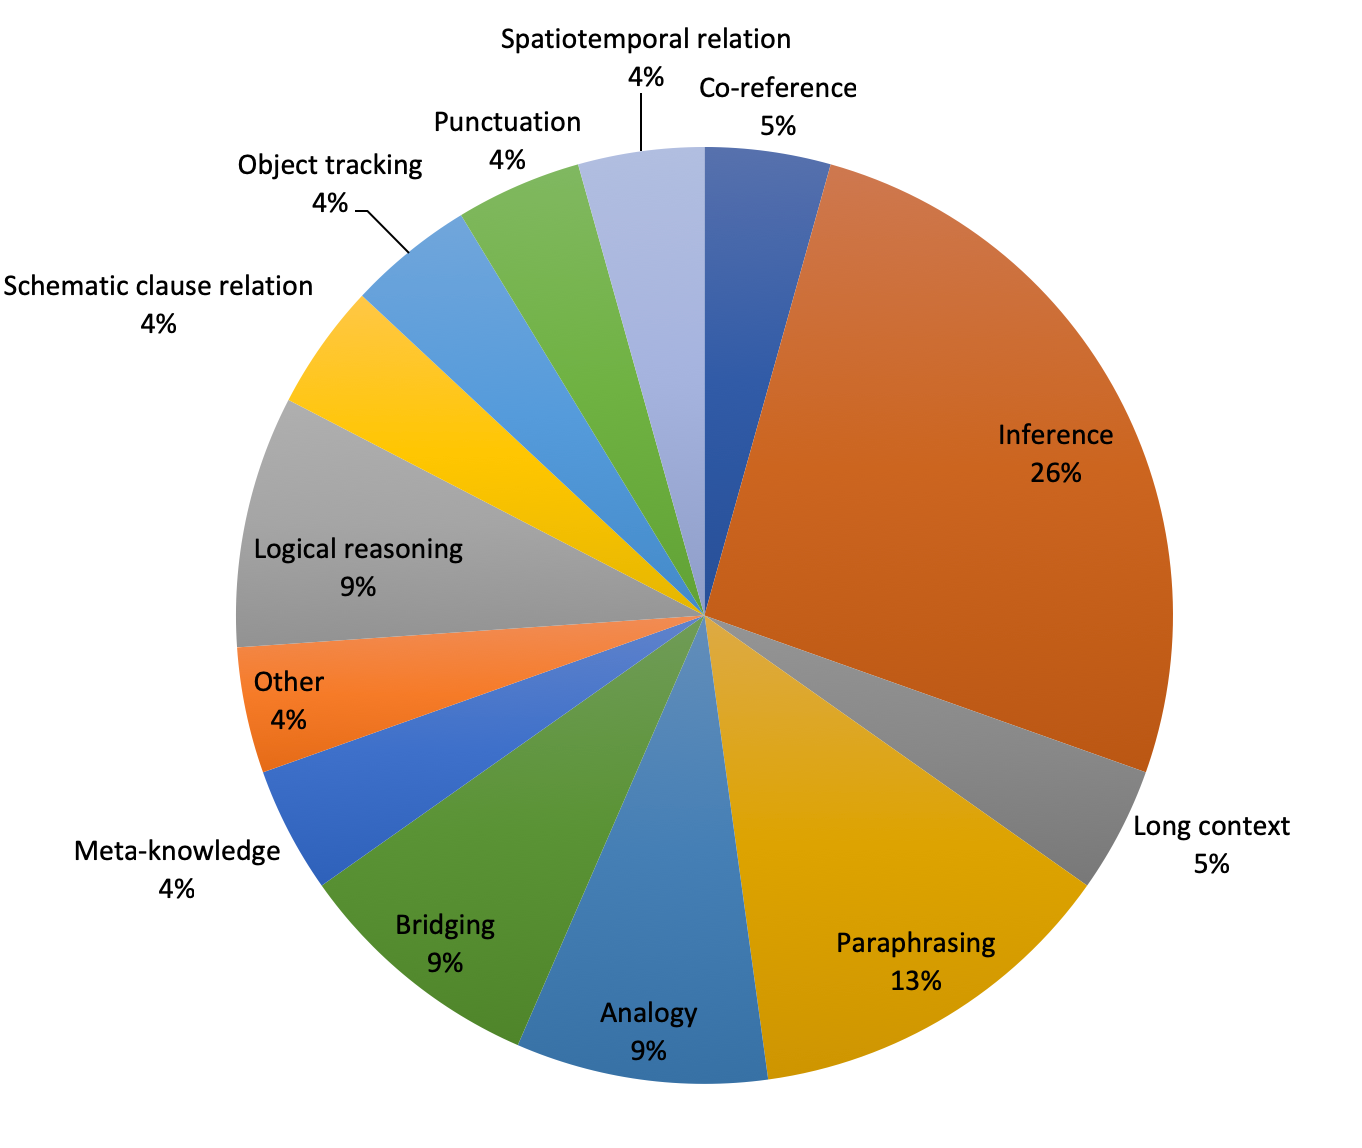
\includegraphics[height=10\baselineskip]{../images/error_types_skills.png}} \quad
     \caption{Errors by types and skills - answerable questions}
  \label{error-types-figure}
\end{figure}


Curiously, we also noticed a handful errors in the ground truth, especially with paragraphs dealing with highly technical topics. Examples include

\begin{enumerate}
\item Nonsensical phrasing: \textit{What are there no longer limitations on since 1990?}
\item Illogical: \textit{What can scales and spring balances measure between two forces by using static equilibrium?} Expected answer: \textbf{forces}
\item Incorrect answers: \textit{What is the force equivalent of torque compared to angular momentum?}  None of the human annotators provide the correct answer, \textbf{momentum}
\end{enumerate}

\begin{table}[htbp]
\tiny
\caption{Examples of error in predictions of answerable questions}
\label{error-types-table}
\tiny Ground truth spans in context are highlighted in \textcolor{blue}{blue}. Key phrases in context and question that are relevant for answering are highlighted in \textcolor{violet}{violet}
\centering
\begin{tabular}
{p{0.5\textwidth}
p{0.2\textwidth}
p{0.2\textwidth}
p{0.1\textwidth}} \\ \toprule

Context 
& Question 
& Prediction 
& Skill-deficiency \\ \midrule

Newton came to realize that the effects of gravity might be observed in different ways at larger distances. In particular, Newton determined that the acceleration of the Moon around the Earth could be ascribed to the same force of gravity if the \textcolor{blue}{acceleration due to gravity} decreased as an inverse square law. Further, Newton realized that the acceleration due to gravity is proportional to the mass of the attracting body. Combining these ideas gives a formula that relates the mass () and the radius () of the Earth to the gravitational acceleration: 
& What is  \textcolor{blue}{gravitational acceleration} proportional to? &  & Paraphrasing \\

An early important political response to the opening of hostilities was the convening of the Albany Congress in June and July, 1754. The goal of the congress was to formalize a unified front in trade and negotiations with various Indians, since allegiance of the various tribes and nations was seen to be pivotal in the success in the war that was unfolding. The plan that the delegates agreed to was never ratified by the colonial legislatures nor approved of by the crown. Nevertheless, the format of the congress and many specifics of the plan \textcolor{blue}{became the prototype for confederation} during the War of Independence. & What was the \textcolor{blue}{importance} of the congress? & to formalize a unified front in trade and negotiations with various Indians & Inference  \\

In England, the period of \textcolor{blue}{Norman architecture} immediately \textcolor{violet}{succeeds} that of the Anglo-Saxon and precedes the Early Gothic. In southern Italy, the Normans incorporated elements of Islamic, Lombard, and Byzantine building techniques into their own, initiating a unique style known as Norman-Arab architecture within the Kingdom of Sicily. & What architecture type came \textcolor{violet}{before} Norman in England? &  & Spatiotemporal relation  \\ 

Bethencourt took the title of King of the Canary Islands, as vassal to Henry III of Castile. In 1418, Jean's nephew Maciot de Bethencourt \textcolor{violet}{sold} the rights to the islands to \textcolor{blue}{Enrique Pérez de Guzmán}, 2nd Count de Niebla. &Who \textcolor{violet}{bought} the rights? &Maciot de Bethencourt & Logical-reasoning  \\ 

For many native populations, the elimination of French power in North America meant the disappearance of a strong ally and counterweight to British expansion, leading to their ultimate dispossession. The Ohio Country was particularly vulnerable to legal and illegal settlement due to the construction of military roads to the area by Braddock and Forbes. Although the Spanish takeover of the Louisiana territory (which was not completed until 1769) had modest repercussions, the British takeover of Spanish Florida resulted in the westward migration of tribes that did not want to do business with the British, and a rise in tensions between the Choctaw and the Creek, historic enemies whose divisions the British at times exploited. The change of control in Florida also prompted most of its \textcolor{violet}{Spanish Catholic population} to leave. \textcolor{violet}{Most} went to \textcolor{blue}{Cuba}, including the entire governmental records from St. Augustine, although some Christianized Yamasee were resettled to the coast of Mexico. &Where did many Spanish Catholic move after British takeover in Florida? &  & Co-reference  \\ 

\bottomrule
\end{tabular}
\end{table}


\begin{wrapfigure}{r}{0.5\linewidth}
  \vspace{-15pt}
\centering
   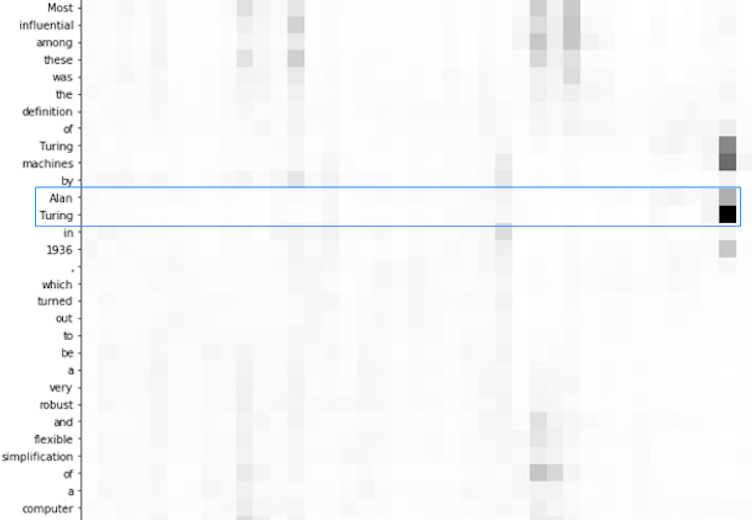
\includegraphics[width=\linewidth]{../images/attention_excerpt.png}
\caption{Attention at work}
\label{attention-excerpt-figure}
\end{wrapfigure}

\textbf{Attention at work:} As expected, whenever a question is answered correctly by the system, the ever-dependable attention mechanism again seems to perform well inside the QANet architecture. We visualized the attention distribution in the last encoder block of the first stacked encoder block in the model encode layer (encoder block 7 of 21). Given the question \textit{Who was the most influential researcher among those grappling with the deficit of work surrounding the complexity posed by algorithmic problems?}, the tokens corresponding to the correct answer, \textit{\{Alan, Turing\}} from the context get the highest levels of attention as shown in Figure~\ref{attention-excerpt-figure}. For the sake of simplicity the figure shows a single head of attention, cropped to fit the page. For the uncropped version, see the appendix. \ref{appendix:a}


\section{Conclusion}
In this work, we implemented the QANet model for machine reading comprehension. We evaluated the model against the SQuAD [2.0] dataset and analyzed the results.  Prior to the recent PCE methods, QANet was the SoTA system for question answering. QANet is a complex model with more than 130 layers. Implementing the architecture correctly in a short span time based on the brief descriptions in the paper was a huge challenge. Our motivation behind choosing this project was to carefully study the key ideas (such as, attention mechanism, pointer networks etc.) from the recent innovations of neural architectures that the QANet is built upon. We hoped to gain hands-on experience by implementing the architecture “from the scratch”. We believe we have accomplished this learning goal. However, due to time constraints, we could not further explore adapting QANet architecture for SQuAD [2.0] dataset.  At the outset, we want to pursue ideas along two different dimensions:
\begin{enumerate}
  \item \textit{Answerability prediction improvements:} Previous works, including the framework supplied as part of the baseline implementation for default final project, usually predict an additional “no-answer” probability to detect unanswerable cases. Given a context of $N$ tokens, this model predicts start/end probabilities for $N+1$ positions. The start/end probabilities in the extra position are used for answerability prediction. Other approaches include adding auxiliary losses to the system \cite{hu2018read+} or encoding the no-answer option within the model \cite{clark2017simple}.
  \item \textit{General accuracy improvements for answerable questions:} Borrowing some ideas from Transformer-XL architecture \cite{dai2019transformerxl} to improve accuracy of QANet, especially for handling long-range dependencies could prove valuable. 
\end{enumerate}	
Further, evaluating against domain-specific datasets such as CliCR \cite{vsuster2018clicr} would be another future direction. 


\subsubsection*{Acknowledgments}
We are immensely grateful to Chris Chute for his help in interpreting the paper, providing guidance in debugging and in finding a critical bug in the persistence of model parameters to disk. We greatly appreciate Abi See for taking time outside the office hours and providing valuable direction. We would also like to thank Stephanie Dong for her help with the Azure.  

\bibliographystyle{plain}
\bibliography{../references/References}

 \cleardoublepage

\appendix
\section{Attention mechanism}
\label{appendix:a}
\begin{figure}[h]
  \vspace{-10pt}
  \centering
  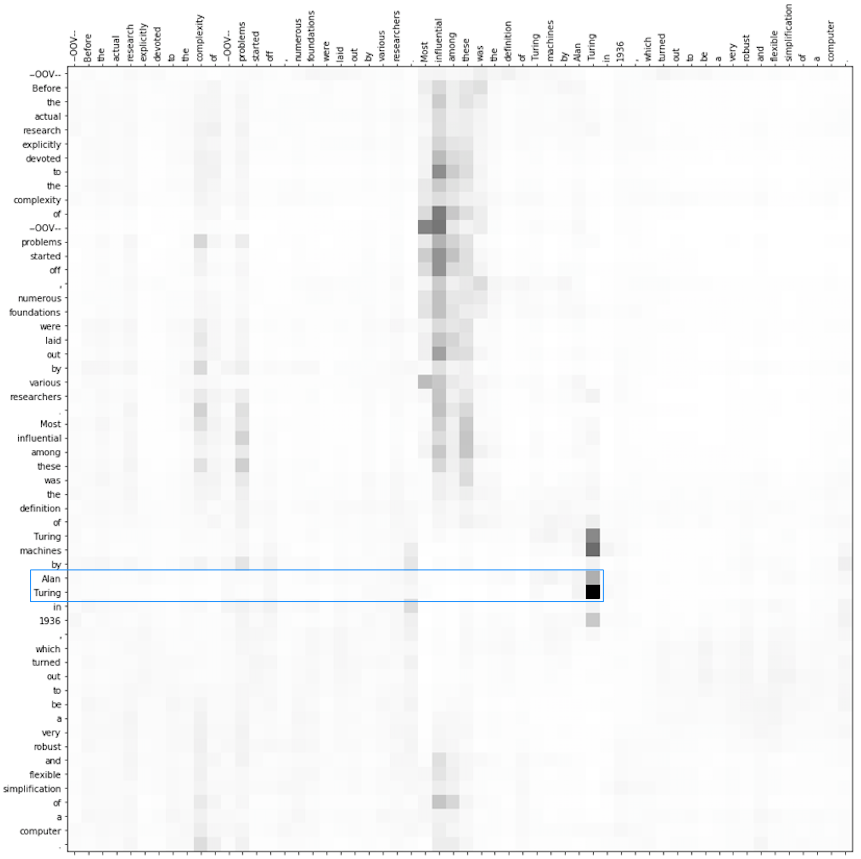
\includegraphics[scale=0.5]{../images/attention.png}
  \caption{Attention mechanism at work}
  \tiny
\textbf{Question:} Who was the most influential researcher among those grappling with the deficit of work surrounding the complexity posed by algorithmic problems?
\textbf{Answer:} Alan Turing
  \label{attention-full-figure}
\end{figure} 


\end{document}